%!TEX root = ../../../thesis.tex

This chapter looks at each of the components within the interface model.
The parameters that govern the behaviour of those components will be discussed, as will methods of measuring those parameters.
The measurements and determined parameters will be presented in the next chapter (\cref{chap:interfaceParameters}).


\section{The Scott-Single Interface Model}


  \begin{figure}
    \centering
    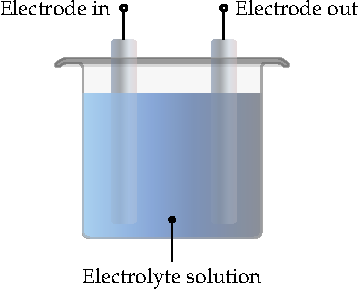
\includegraphics{content/pt2/07-InterfaceModel/graphics/electrode-electrolyte}
    \caption{\label{fig:electrode-electrolyte}Electrodes submerged in an electrolyte solution, such a system can be described by the Scott-Single Interface Model.}
  \end{figure}

  Jonathan Scott and Peter Single published an electrical model of an implantable electrode array in saline in 2013 \cite{ScottSingle2013}.
  The intention of that model was to simulate the electrical impedance that a medical implant device would be subjected to once implanted into a human spinal cavity.
  It is also general enough to use in any situation where electrodes are placed in an electrolyte solution, such as depicted in \cref{fig:electrode-electrolyte}.

  \begin{figure}
    \centering
    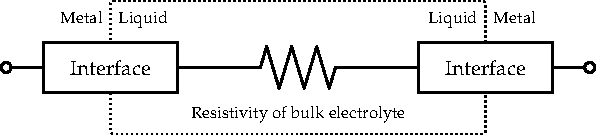
\includegraphics{content/pt2/07-InterfaceModel/graphics/simpleElectrodeElectrolyteModel}
    \caption{\label{fig:pt2-simpleElectrodeElectrolyteModel}Connection diagram of two electrodes (with their interface models) connected together by the resistivity of an electrolyte solution.}
  \end{figure}
  The model comes in two parts: the electrode interface, and the resistivity of the electrolyte's bulk.
  \Cref{fig:pt2-simpleElectrodeElectrolyteModel} shows the general electrical configuration of such an electrode-electrolyte system.
  It shows that there are two interfaces per system, and that the liquid side of those two interfaces are joined electrically by the resistance of the electrolyte's bulk resistivity.
  The metal side of the interfaces is what the rest of the circuit would connect to.
  First, the interface model will be explained.


%  \subsection{Breakdown of model components}

  \begin{figure}
    \centering
    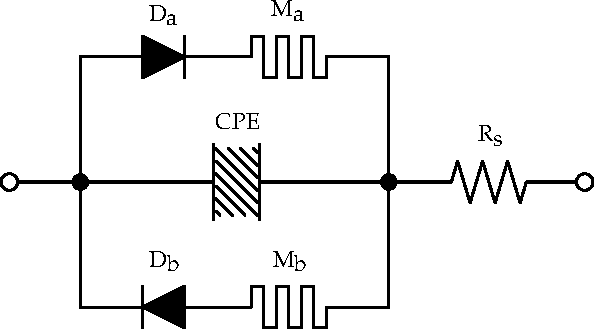
\includegraphics{content/pt2/07-InterfaceModel/graphics/interfaceSchematic}
    \caption{\label{fig:pt2-interfaceSchematic}Electrical schematic of the electrode-electrolyte interface}
  \end{figure}

  The full interface model is represented schematically by \cref{fig:pt2-interfaceSchematic}.
  It represents the transition between the metal of the electrode and the liquid of the electrolyte.
  The model used throughout this thesis is a slightly simplified version of \cref{fig:pt2-interfaceSchematic} in that the memristors (elements M\textsubscript{a} and M\textsubscript{b}) have been removed.

  % The Scott-Single interface is modelled by the circuit shown in \cref{fig:pt2-interfaceSchematic}.
  % Each of the components and their functions will be explained in the coming sections.
  % It is important to realise that this model only represents a single interface between metal and electrolyte.
  % By itself it is incapable of simulating any useful electrode/electrolyte system.
  % For that, a minimum of two interfaces must be used - one as a cathode and one as an anode.
  % Additionally, some model of the electrolyte resistivity needs to connect the two interfaces.


  % \Cref{fig:pt2-simpleElectrodeElectrolyteModel} shows the smallest/simplest use of the interface model.
  % This configuration represents two electrodes placed in an electrolyte solution.
  % It allows simulation of impedance between those electrodes and can be connected to other electronic circuits.
  % A model like this is only valid for a two electrode system.
  % Because the electrode array in our application has eight electrodes, the model is more complex.
  % In full, that model will have eight electrode interfaces and a resistor network connecting each interface.


  \subsection{Inter-electrode resistivity (resistor network)}


    Modelling the resistance between two electrodes in a fixed geometry situation is simply a matter of inserting an appropriately sized resistor between the two interfaces.
    The resistance is dependent on the electrolyte's conductivity, the combined surface area of the two electrodes and the distance between them.
    Modelling an electrode array, such as the St. Jude Medical - Octrode, is more complex as it requires a resistor network to describe the inter-electrode resistances.
    An illustration of an Octrode is presented as \cref{fig:StJudeOctrode_Labelled}.

    \begin{figure}
      \centering
      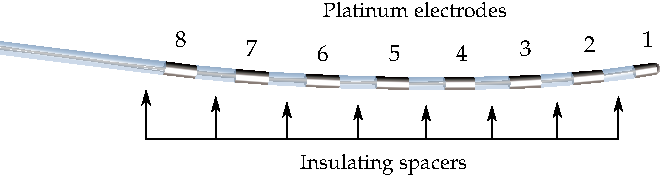
\includegraphics{content/pt2/07-InterfaceModel/graphics/StJudeOctrodeDiagram}
      \caption{\label{fig:StJudeOctrode_Labelled}St. Jude Medical Octrode. An eight electrode array commonly used in spinal stimulation implants. The electrode numbering shown here will be used throughout this work.}
    \end{figure}

    % Edit checkpoint 2015-09-17 20:23

    Scott and Single created a resistor network for modelling the electrolyte conductivity based on the geometry of the electrodes and the resistivity of the electrolyte.
    By sectioning the surrounding liquid into cylindrical volumes they calculated the equivalent resistance between those volumes in both radial and longitudinal planes.
    The radii of the volumes double at each layer which correspond to a fixed radial resistance between each layer.
    There are two different radial resistances: one for the rings expanding from the insulating spacers, and one for those expanding from the electrode cylinders.
    The two alternate due to each electrode being separated by an insulating spacer.
    The longitudinal resistances quarter in size with each ring layer and after the last radial resistor each node is shorted together.
    The full mesh for the eight electrode array is five layers deep with three rows of padding at each terminating end, totalling two hundred and five resistors in total.
    \Cref{fig:pt2-ResistorMesh} shows the resistor network schematic.
    Further details of how the mesh geometry and resistor values were calculated can be found in \cite{Scott2014}.

    The parameters that describe the resistor mesh are:
    \begin{itemize}
    \item $R_{eri}$ - The initial resistance placed radially from an electrode.
    \item $R_{sri}$ - The initial resistance placed radially from a spacer.
    \item $R_{li}$ - The longitudinal resistance.
    \item Depth - Number of layers between the electrode/spacer and the common end node in the ladder
    \item Padding - Number of additional spacing rows to be added to each end of the mesh.
    \end{itemize}

    \begin{figure}
      \centering
      \includegraphics{content/pt2/07-InterfaceModel/graphics/resistorMesh}
      \caption{\label{fig:pt2-ResistorMesh}Resistor mesh used to model the electrical resistance between interface pairs. $R_{li}$ is longitudinal resistance, $R_{sri}$ and $R_{eri}$ is the radial resistance for the spacers and electrodes respectively, and $I$ is an interface.}
    \end{figure}


  \subsection{Interface series resistance (resistor)}


    The series resistor at the right hand side of the model schematic (labelled $R_{S}$) represents the purely resistive component of the interface's impedance.
    As it is in series with all other components in the interface model, there is no way for charge to cross the interface without encountering this resistance.
    The parameter used to denote the interface's series resistance is:
    \begin{itemize}
      \item $R_S$ -- The series resistance of the interface
    \end{itemize}

  \subsection{Polar/double-layer effects (constant phase element)}

    At the centre of the model is the constant phase element (CPE), or fractional pole capacitor.
    A CPE is a device that behaves like a cross between a capacitor and a resistor.
    They are primarily used to describe the capacitance of double layer interfaces, the function it serves in this model.
    It is capacitive in the sense that voltage leads current, but by an amount less than \SI{90}{\degree}.
    Mathematically, the \SI{90}{\degree} angle between sinusoidal voltages and currents in a capacitor is a result of the capacitors current being
    \begin{equation}
    I(t) = C \times \frac{dV(t)}{dt}
    \label{eqn:currentVoltageInCapacitor}
    \end{equation}
    When $V(t)$ is a sine wave, this becomes
    \begin{align}
      I(t) &= C \times \frac{d Sin(t)}{dt}
      I(t) &= C \times Cos(t)
    \end{align}
    A capacitor's impedance is \SI{-90}{\degree} out of phase because the angle between sine and cosine is \SI{-90}{\degree}, the angle between the current and voltage in the previous equation.
    A CPE on the other hand has a phase angle somewhere \emph{between} 0 and \SI{-90}{\degree}.
    This requires a fractional differentiation of \cref{eqn:currentVoltageInCapacitor} by doing:
    \begin{equation}
      I(t) = C \frac{d^n V(t)}{dt^n}
    \end{equation}
    where n is a non-integer number.
    Partially applied differential is uncommon outside of pure mathematics.
    % This requires a fractional differentiation of $I(t) = C \times \frac{d^n V(t)}{dt^n}$, something uncommon outside of pure mathematics.
    As a consequence of having a current/voltage relationship of less than \SI{90}{\degree}, a CPE's impedance magnitude decays at a rate lower than 20\ dB/decade.

    SPICE, or any other commonly used circuit simulators, do not support fractional pole capacitors so entering one into the model will require building it up from discrete components.
    \begin{figure}[h]
      \centering
      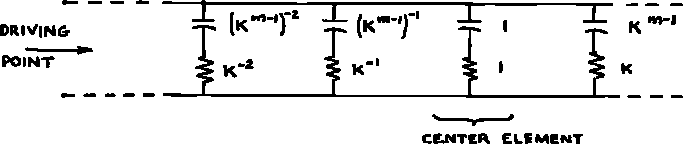
\includegraphics{content/pt2/07-InterfaceModel/graphics/Morrison-RC}
      \caption{\label{graph:pt2-morrisonCPE}Ralph Morrison's implementation of a constant phase element using an infinite array of resistor-capacitor pairs (taken from Morrison's paper -- \cite{Morrison1959}).}
    \end{figure}
    In 1959, Morrison demonstrated a way of creating constant phase elements from an infinite array of resistor-capacitor (RC) pairs \cite{Morrison1959}.
    One of Morrison's implementations of a constant phase element is presented as \cref{graph:pt2-morrisonCPE}.
    In that implementation, each parallel branch has precisely chosen resistor and capacitor values such that when summed together the impedance magnitude versus frequency is a constant slope, i.e., the impedance does not flatten at a particular frequency as it would with a single RC pair.
    Creating any element comprised of an infinite number of sub-elements is not possible, however by selecting only those elements that contribute to the bandwidth of interest the result is the same within the selected frequency window.
    Using that method and selecting only RC pairs with a cut-off frequency in the range of \SI{1}{\milli\hertz} to \SI{1}{\mega\hertz}, a practical CPE element is created.

    \begin{figure}
      \centering
      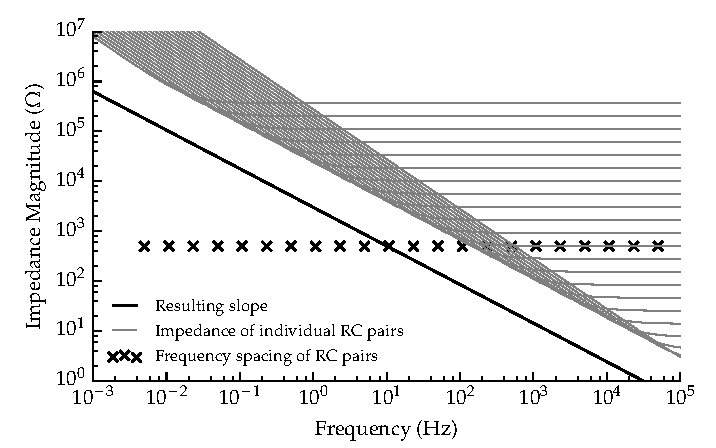
\includegraphics{content/pt2/07-InterfaceModel/graphics/graph_cpe_creation}
      \caption{\label{graph:pt2-cpe_creation}Graph showing how a non \SI{-20}{\decibel} per decade slope can be constructed from a series of \SI{-20}{\decibel} per decade low-pass filters}
    \end{figure}

    \Cref{graph:pt2-cpe_creation} shows the individual contributions from each RC branch in an implementation of a CPE.
    Each grey trace represents a single RC branch in the CPE element, each acting as a low-pass filter.
    The value of the resistor in each branch is evident by the vertical spacing of the traces, clearly visible at the right-hand side of the graph.
    The branches in this particular example have been spaced in the frequency domain at a density of three per decade, as marked by the black crosses.
    This means that per decade of frequency, there are three corner frequencies, each relating to an RC pair.
    Because each of there branches are in parallel, the total response of the CPE is the sum of each branch.
    That response is shown as the black trace on the graph.
    The critical observation is that the slope of the resulting trace is not the same as each of the individual branches.
    This allows the CPE to behave fractionally as a capacitor, being anywhere between resistive (horizontal response) and capacitive (\SI{20}{\decibel}/decade slope).

    The CPE represents readily reversible reactions, polar reorientation, and ionic repulsion and attraction between the electrode's surface and the electrolyte.
    It is capacitive in nature because each of these mechanisms store charge, which can be drawn back by reversing the applied electromotive force.
    Parameters used to describe the behaviour of the CPE are:
    \begin{itemize}
      \item $m$ -- Used to select resistor-capacitor pairs in each branch and ultimately determines the slope of the CPE's frequency response
      \item $k$ -- Spacing, or density, of R-C branches with frequency
      \item $|Z|$ @ \SI{1}{\kilo\hertz} -- Sets the vertical position of the magnitude of CPE's frequency response at a known frequency
    \end{itemize}

    % Edit checkpoint 2015-09-17 21:17


  \subsection{Faradaic reactions (diodes)}


    If the voltage placed across the interface is kept within certain limits, the CPE and series resistance ($R_{S}$) would be all that is necessary to accurately mimic a single electrode-electrolyte interface.
    But once the electric potential across the interface becomes high enough, Faradaic reactions will occur at the electrode's surface.
    Faradaic reactions are reactions involving charge transfer, adding ionised species to the electrolyte and often producing gas.
    Gas, or any new species, is disastrous in an implanted setting as this causes damage to the implant's host.
    Possible Faradaic reactions between saline and platinum electrodes are:
    \begin{eqnarray}
        Pt + H_{2}O &\Leftrightarrow& PtO + 2 H^{+} + 2 e^{-}\\
        PtO + H_{2}O &\Leftrightarrow& PtO_{2} + 2 H^{+} + 2e^{-}\\
        Pt + H^{+} + e^{-} & \Leftrightarrow & Pt-H\\
        Pt + H_{2}O + e^{-} &\Leftrightarrow& Pt-H+OH^{-}
    \end{eqnarray}

    The electrical current density through an electrode as a function of electrode overpotential and the cathodic and anodic reactions occurring at each electrode is given by:
    \begin{equation}
      i_{net} = i_{0} \left\{ \frac{[O]_{(0,t)}}{[O]_{\infty}}e^{-\alpha_{c}nf\eta} - \frac{[R]_{(0,t)}}{[R]_{\infty}}e^{(1-\alpha_{c})nf\eta}\right\}
      \label{eqn:pt-2_butlerVolmerEquation}
    \end{equation}
    % \Cref{eqn:pt-2_butlerVolmerEquation} describes electrical current density through an electrode as a function of electrode overpotential and the cathodic and anodic reactions occurring at each electrode.
    This is the current-overpotential equation and is derived from the more general Butler-Volmer equation \cite{Merrill2005,ScottSingle2013}.
    In \cref{eqn:pt-2_butlerVolmerEquation}, $i_{net}$ is the net Faradaic current across the electrode-electrolyte interface,
    $i_{0}$ is the exchange current density,
    $[O]_{(0,t)}$ and $[R]_{(0,t)}$ are the oxidant and reductant concentrations at the electrode surface as a function of time,
    $[O]_{\infty}$ and $[R]_{\infty}$ are concentrations of reactant in the bulk electrolyte,
    $\alpha_{c}$ is the cathodic transfer coefficient (approximately 0.5),
    $n$ is the number of moles of electrons per mole of reactant oxidised,
    $f$ is Faraday's constant divided by the product of the gas constant and the absolute temperature ($F/RT$),
    and $\eta$ is the electrode overpotential.
    This equation describes the forward and reverse electrical current through an electrode by separating the forward and reverse reactions: oxidisation and reduction.
    \begin{equation}
      I = i_0 e^{V_D / n V_T}
      \label{eqn:pt-2_diodeEquation}
    \end{equation}
    Taking a single half of the equation, either the reduction or oxidisation, yields an equation that is similar to that for the current through a diode; an observation made by McAdams and utilised in the Scott-Single model \cite{McAdams1995}.
    The standard diode equation is shown as \cref{eqn:pt-2_diodeEquation}, where
    $I$ is the current through the diode,
    $i_0$ is the diode saturation current,
    $V_D$ is the potential across the diode,
    $n$ is the diode's ideality factor,
    $V_T$ is the thermal voltage (defined as the product of Boltzmann's constant and temperature divided by the charge on an electron).
    The parameters used to describe the behaviour of the diode are:
    \begin{itemize}
      \item $i_0$ -- the diode's saturation current
      \item $n$ -- the diode's ideality factor
    \end{itemize}
    The diodes themselves can not account for the relative abundance of reactants for the redox reactions ($[O]_{(0,t)}/[O]_{\infty}$ and $[R]_{(0,t)}/[R]_{\infty}$ from \cref{eqn:pt-2_butlerVolmerEquation}), this needs to be considered separately and is discussed next.


  \subsection{Chemical species depletion (memristors)}


    \begin{figure}[h]
      \centering
      \includegraphics{content/pt2/07-InterfaceModel/graphics/memristorSymbol}
      \caption{\label{fig:pt2-memristorSymbol}Electrical symbol of a memristor, as is used in the original electrode-electrolyte interface model}
    \end{figure}

    A memristor is a two port device that sets its resistance based on its own history.
    The resistance can either depend on the integral over time of the voltage placed across it or the total charge passed through the device \cite{Kvatinsky2012}.
    Its name is a portmanteau of the word `memory' and `resistor' owing to its use of memory to set its resistance~\cite{Williams2008}.

    The memristive device models species depletion in the electrolyte as an increase in resistance in the diode/memristor branch in proportion to the integral of charge passed through the branch.
    As the specific Faradaic reaction proceeds, it consumes the reactants from the electrolyte bulk until eventually none is left.
    Increasing the resistance in series with a conducting diode has the effect of removing that diodes current path from the circuit, simulating the depletion of reactants of the modelled reaction.

    Memristors were removed from the model used in this work as they added complexity that would yield little in the way of research outcomes.
    The diodes are only used to model the \emph{onset} of Faradaic conduction, which is the most relevant parameter of the Faradaic modelling.
    Once these reactions begin, the electrode overpotential has been pushed too far and there is little to be gained from knowing how far the reaction can be run until the reactants have been depleted.
    In an implanted setting it is likely that the electrolyte will circulate throughout the body, bringing new reactants to the electrode's surface over time.
    Species depletion is likely to be a slow process, dependent on the electrolyte volume and species concentration.

    \begin{figure}
      \centering
      \includegraphics{content/pt2/07-InterfaceModel/graphics/interfaceSchematic_noMemristive}
      \caption{\label{fig:pt2-interfaceSchematic_noMemristive}Electrical schematic of the electrode-electrolyte interface without memristors (as used throughout this thesis)}
    \end{figure}

    \Cref{fig:pt2-interfaceSchematic_noMemristive} shows the interface model used throughout the remainder of this thesis.
    Although it is slightly different to the Scott-Single interface model, the other parameters are unaffected by the removal of these elements.

    % Edit checkpoint 2015-09-17 21:31


\section{Phosphate Buffered Saline as an Electrolyte}


  The model has been fitted to phosphate buffered saline (PBS) because it was the closest artificial representation of human spinal fluid at the time of writing.
  Engineers at Saluda used a concentration one-tenth that of a standard solution of PBS as a test solution for their spinal implants.
  It was not understood how well the one-tenth concentration matched cerebrospinal fluid electrically, which is the main question this work sets out of answer.
  The ingredients used to make the stock solution of standard PBS are given in \cref{tab:pt2-PBS-recipe} and the procedure for mixing up derivative solutions are:
  \begin{enumerate}
    \item Weigh out dry ingredients and combine in a large stock bottle.
    \item Add \SI{800}{\milli\litre} of distilled water and stir until all solids have dissolved.
    \item Measure the pH and adjust to 7.4 by adding HCl.
    \item Continue to add distilled water until the stock solution occupies a volume of \SI{1000}{\milli\litre}.
  \end{enumerate}

  \begin{table}
    \centering
    \begin{tabular}{r | r | c}
      Ingredient & Quantity & Unit \\
      \hline
      H$_2$O & 1000 & ml \\
      NaCl & 8.00  & g  \\
      KCl  & 0.20  & g  \\
      Na$_2$HPO$_4$ & 1.44 & g \\
      KH$_2$PO$_4$  & 0.24 & g \\
    \end{tabular}
    \caption{\label{tab:pt2-PBS-recipe}Ingredients used to produce one litre of stock solution of phosphate buffered saline.}
  \end{table}

  \begin{table}
    \centering
    \begin{tabular}{r | r | c}
      Stock (ml) & Water (ml) & Final Concentration \\
      \hline
      700.0 &   0.0 & 1.00X \\
      350.0 & 350.0 & 0.50X \\
      175.0 & 525.0 & 0.25X \\
       70.0 & 630.0 & 0.10X \\
       35.0 & 665.0 & 0.05X \\
       17.5 & 682.5 & 0.025X\\
    \end{tabular}
    \caption{\label{tab:pt2-PBS-concentration}Final dilutions of stock to create six \SI{700}{\milli\litre} solutions ranging from 0.025X to 1X standard PBS concentration.}
  \end{table}

  Six bottles ranging in concentration from full strength (1.0X) to one-fortieth (0.025X) of the stock solution were created by dilution.
  \Cref{tab:pt2-PBS-concentration} shows the volumetric ratios used to create those six concentrations of PBS, which are then used to fit the model parameters to.

  % Edit checkpoint 2015-09-19 09:02


\section{Parameter Extraction Methods}


  The interface model has six parameters (plus five supporting parameters) that are used to set the behaviour of each component in the model.
  Finding suitable values for each parameter is essential to ensure the final model is a good representation of the system it mimics.
  Critical to finding those suitable values are the methods used to extract measurement data relating to different parts of the interface model.
  A divide-and-conquer approach is taken wherever possible so that parameter measurements for specific elements are isolated from other elements in the model.
  The following section describes those measurements and explains how they isolate the properties of each component.

  Scott and Single found a set of parameters that described the Octrode in a one-tenth concentration solution of phosphate buffered saline (PBS).
  In this section I create six different solutions of PBS ranging in concentration from 1.0x to 0.025x the concentration of a standard PBS solution.
  I extend the Scott-Single model to work over a range of concentrations by expressing relevant parameters in terms of a dependent variable - PBS concentration.


  \subsection{Inter-electrode resistivity}


    In order to find the parameters of any elements within the electrode-electrolyte interface it is first necessary to find the inter-electrode resistances.
    The reason is that no element within the interface can be measured without a resistive contribution being added by the electrolyte itself.
    To model the restive contribution from the electrolyte bulk, a resistor mesh is created that connects each electrode together.
    To determine the resistances used in that resistor mesh, I use the same method as was used by Scott and Single \cite{Scott2014}.
    Once those resistances are accounted for, the behaviour of components in the interface can be calculated from measurements that include those inter-electrode resistances by subtracting out that expected contribution.

    \begin{figure}
      \centering
      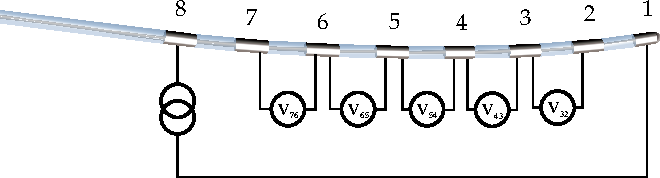
\includegraphics{content/pt2/07-InterfaceModel/graphics/TransimpedanceMeasurements_Stim81}
      \caption{\label{fig:pt2-transimpedanceMeasurementDiagram_81Stim}Schematic of trans-impedance measurements where electrodes eight and one are driven and the remainder are used in voltage differential measurements.}
    \end{figure}

    \begin{figure}
      \centering
      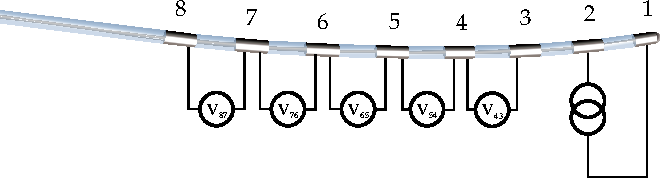
\includegraphics{content/pt2/07-InterfaceModel/graphics/TransimpedanceMeasurements_Stim21}
      \caption{\label{fig:pt2-transimpedanceMeasurementDiagram_21Stim}Schematic of trans-impedance measurements where electrodes two and one are driven and the remainder are used in voltage differential measurements.}
    \end{figure}

    Scott and Single measure the trans-impedance of the eight electrodes submerged in the electrolyte solution.
    This works by passing a stimulus current between two electrodes while measuring voltage differentials between pars of non-stimulus carrying electrodes.
    Data from those measurements is then tabulated so that each row contains the AC current driven between the two stimulus electrodes and the voltage measured between a pair of non-driven electrodes.
    By measuring the voltage across pairs of non-driven electrodes using a suitably high impedance measurement, those measurements will correspond to the voltage difference in the electrolyte.
    For this method to work it is assumed that the current passing through each non-driven interface is zero, and therefore no voltage is dropped between the electrode's metal and the electrolyte solution.
    It is for this reason that voltage differentials can not be measured on any of the stimulus electrodes.
    \Cref{fig:pt2-transimpedanceMeasurementDiagram_81Stim,fig:pt2-transimpedanceMeasurementDiagram_21Stim} show the two measurement configurations used to collect trans-impedance data.
    Those trans-impedance results are recreated using a simulated mesh of resistors with fitted values to the three resistor parameters.
    Optimisation routines can find the three values which produce the mesh with closest match to the measured values.
    The source of parameter values for the mesh are given in \cref{tab:pt2-parameterDesc-ResistorMesh}.
    A mesh with those values of padding and depth, and made to fit between eight electrodes, contains 205 resistors.


    \begin{table}
      \begin{center}
        \begin{tabular} {r | l}
          Parameter & Determined from:\\
          \hline
          $R_{eri}$ & optimised fit via SPICE simulation\\
          $R_{sri}$ & optimised fit via SPICE simulation\\
          $R_{li}$ & optimised fit via SPICE simulation\\
          Padding & previous value of 3 rows used (from Scott \& Single)\\
          Depth & previous value of 5 layers used (from Scott \& Single)
        \end{tabular}
      \end{center}
      \caption{\label{tab:pt2-parameterDesc-ResistorMesh}Parameters determined by an optimised fit between a simulated mesh and transimpedance measurements.}
    \end{table}

    % Edit checkpoint 2015-09-19 09:28


  \subsection{Constant phase element \& series resistance}


    \begin{figure}[h]
      \centering
      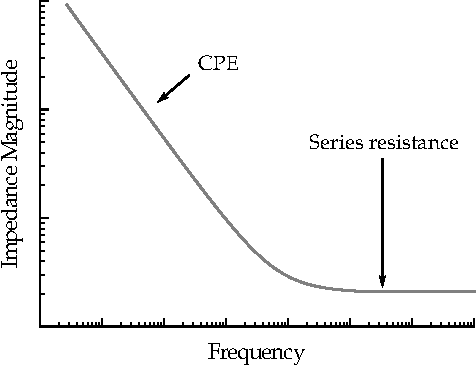
\includegraphics{content/pt2/07-InterfaceModel/graphics/graph_cpePlotGeneral}
      \caption{\label{fig:pt2-graph_cpePlotGeneral}Schematic log-log plot of frequency vs impedance magnitude of a single interface and inter-electrode impedance. The response of the CPE and that of the total series resistance is separated in the frequency domain.}
    \end{figure}
    By accounting for the value of resistance seen between electrodes it is now possible to probe deeper into the interface model.
    Calculation of both the CPE and the series resistance ($R_S$) is made via impedance spectroscopy methods.
    It is possible to use frequency to separate the responses of the CPE from interface's series resistance.
    The impedance of the CPE dominates below \SI{10}{\hertz}, where its slope and magnitude can be determined.
    At higher frequencies, greater than \SI{1}{\kilo\hertz}, the series resistance of both the interface ($R_S$) and the previously determined inter-electrode resistance is evident.
    This separation of responses is illustrated in \cref{fig:pt2-graph_cpePlotGeneral}.
    Subtracting the inter-electrode resistance, determined previously, from the measured resistance yields the interface's series resistance ($R_S$).
    Parameters for the CPE, such as slope and vertical position, are determined from the low frequency part of the trace where the slope is not disturbed by resistive behaviour.
    The parameter $m$ determines the slope of the created CPE, but is not itself a direct measure of slope, i.e., it is used to pick values of resistance and capacitance in each branch in the CPE, which then determine the resulting slope.
    Parameters for the CPE and series resistance are summarised in \cref{tab:pt2-parameterDesc-CPE}.

    \begin{table}
      \begin{center}
        \begin{tabular} {r | l}
          Parameter & Determined from:\\
          \hline
          $k$ & previous value of 3 branches used (from Scott \& Single)\\
          $m$ & determined from the slope of |Z| vs. frequency response\\
          |Z| @ \SI{1}{\hertz} & impedance magnitude at \SI{1}{\hertz}\\
          $R_S$ & impedance at high frequency (\SI{10}{\kilo\hertz}) end of the trace
        \end{tabular}
      \end{center}
      \caption{\label{tab:pt2-parameterDesc-CPE}Parameters describing CPE behaviour and interface series resistance ($R_S$) as determined using impedance spectroscopy based measurements of electrode-electrolyte interface.}
    \end{table}


  \subsection{Faradaic current}


    Measurement of electrical currents associated with Faradaic reactions requires increasing the electrode overpotential until reactions at the electrode's surface begin.
    Those currents then increase exponentially with increasing electrode overpotential.
    Scott and Single used a triangular voltage stimulus as a means to identify the onset of Faradaic conduction at the interface.
    The triangular wave is equivalent to a constant ramp-up and ramp-down of voltage placed across the interface.
    Current flowing into a capacitor is given by:
    \begin{equation}
      I(t) = C \times \frac{dV(t)}{dt}
      \label{eqn:current_in_a_capacitor}
    \end{equation}
    When $\frac{dV(t)}{dt}$ is a constant, as is the case for a linear ramp voltage stimulus, the current is also constant.
    We make the assumption here that fractional differentiation of \cref{eqn:current_in_a_capacitor}, as in the case of a CPE, will give the same relationship between voltage and current.
    By slowly ramping the electrode overpotential the current draw should be constant up to a point after which it becomes exponential.
    The voltage corresponding to the point at which the current draw becomes exponential will be used to determine the onset of Faradaic conduction.
    That point, together with the rate of growth, would then be used to fit values for $i_0$ and $n$.
    The parameters $i_0$ and $n$ are the diode's saturation current and ideality factor respectively, as summarised in \cref{tab:pt2-parameterDesc-Diode}.
    Problems arose with those measurements, discussed in the next chapter, which showed the behaviour of the CPE was less predictable than expected.

    \begin{table}
      \begin{center}
        \begin{tabular} {r | l}
          Parameter & Description \\
          \hline
          $i_0$ & optimised fit of threshold voltage to measured curve\\
          $n$ & optimised fit of growth rate to measured curve
        \end{tabular}
      \end{center}
      \caption{\label{tab:pt2-parameterDesc-Diode}Parameters determined from fitting diode parameters to measured response of Faradaic current.}
    \end{table}

    % Edit checkpoint 2015-09-19 10:11